
\chapter{Joints and links} \label{sec:jointsandlinks}


\paragraph{Joint and link numbering in Fanuc 210F} \label{sec:JointLinkNumbering}
The numbering scheme presented in \fullref{sec:NumJointLink} can be applied to the Fanuc 210F (see  \cref{fig:LinksANDJoints210F}). 


\begin{figure}[H]
	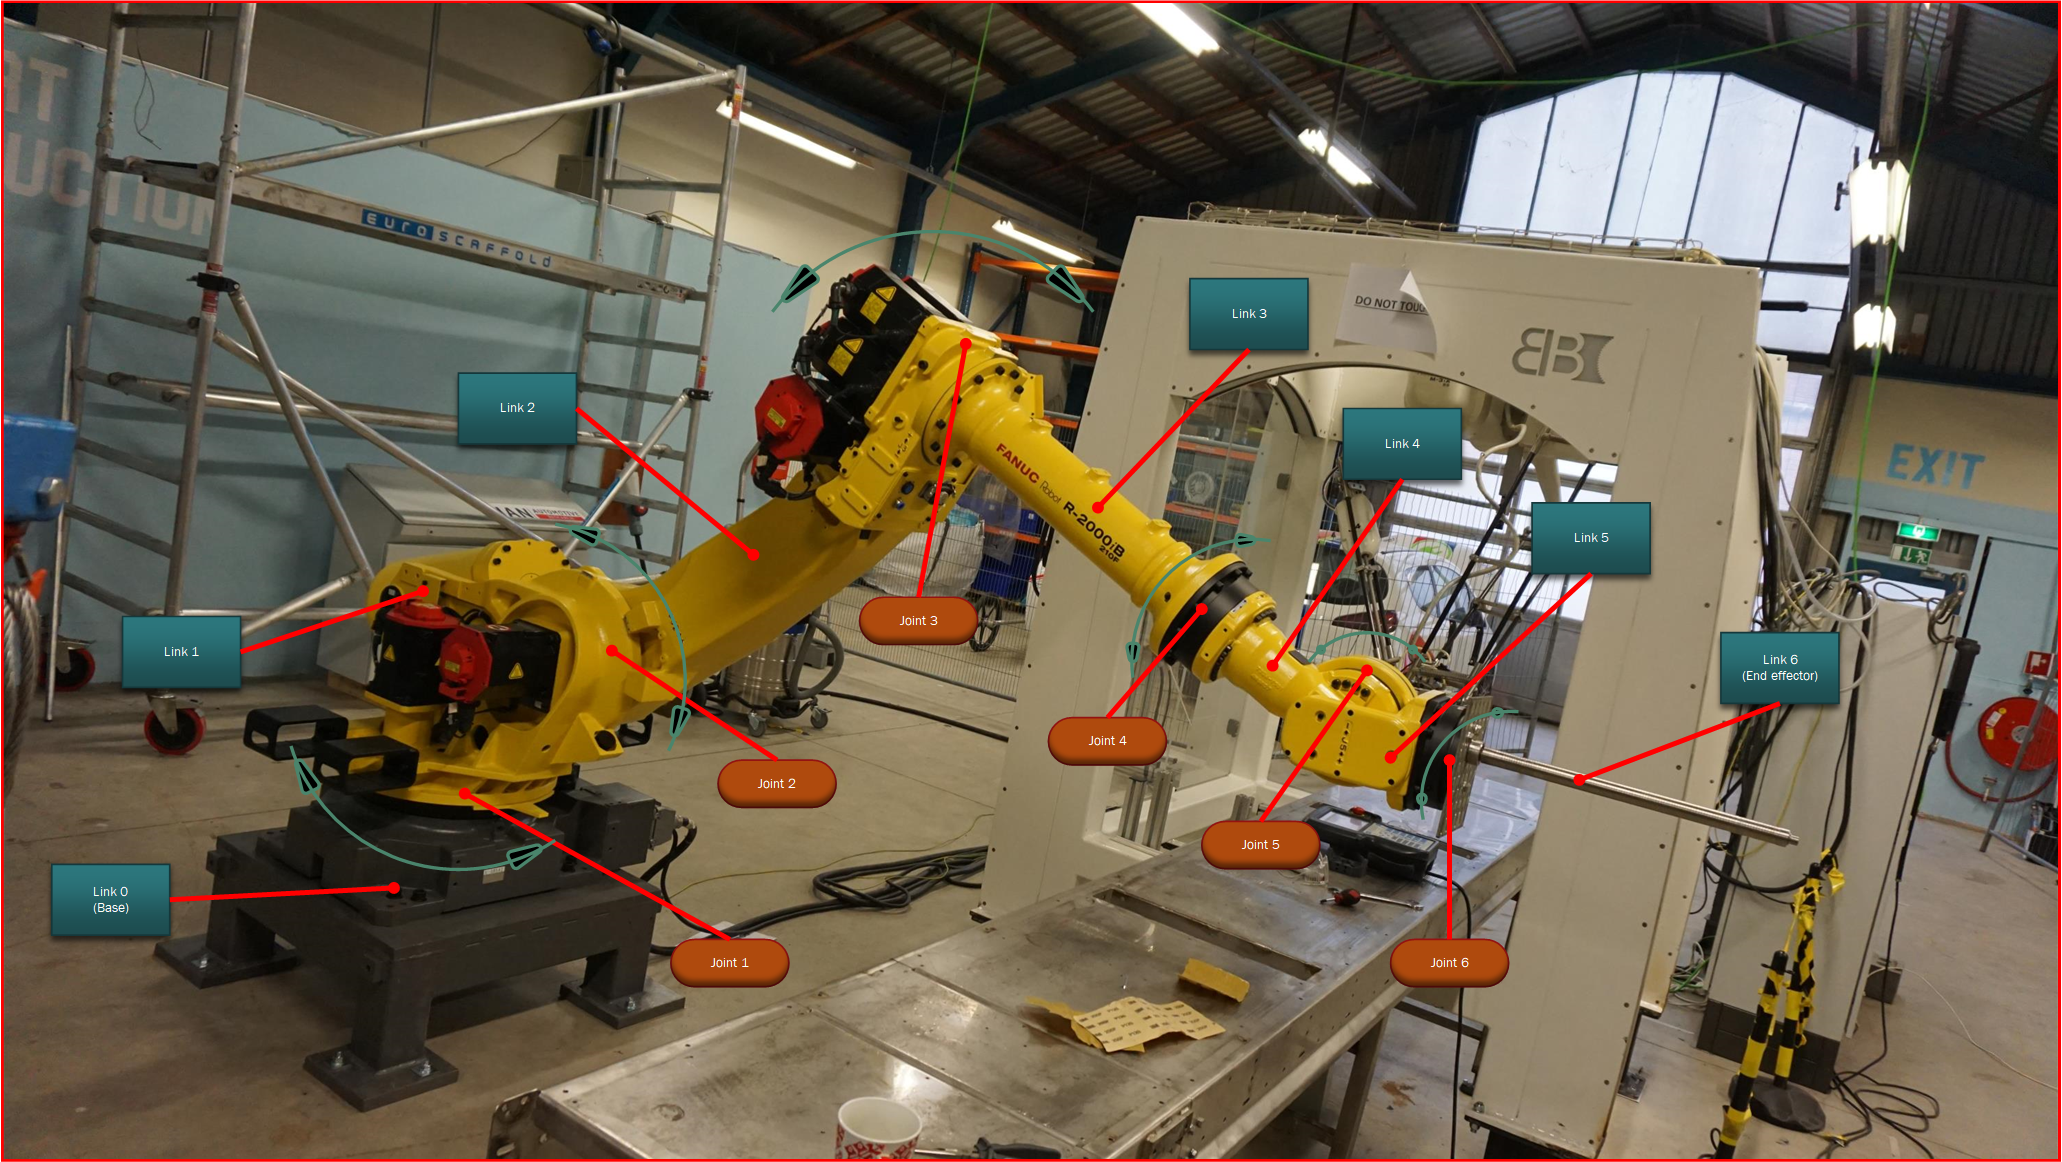
\includegraphics[
	width=1\linewidth,
	center,
	keepaspectratio,
	]{linksANDjoints/linksAndJoints}
	\caption{Links (turquoise) and joints (orange) in the FANUC 210F}
	\label{fig:LinksANDJoints210F}
\end{figure}

\paragraph{\textbf{\gls{z_i}} axes in Fanuc 210F}
As described in \fullref{par:z_iAxesAssign}, the $\gls{z_i}$ axes can be attached to the Fanuc 210F (see figure \ref{fig:zi_Axes}).


\begin{figure}[H]
	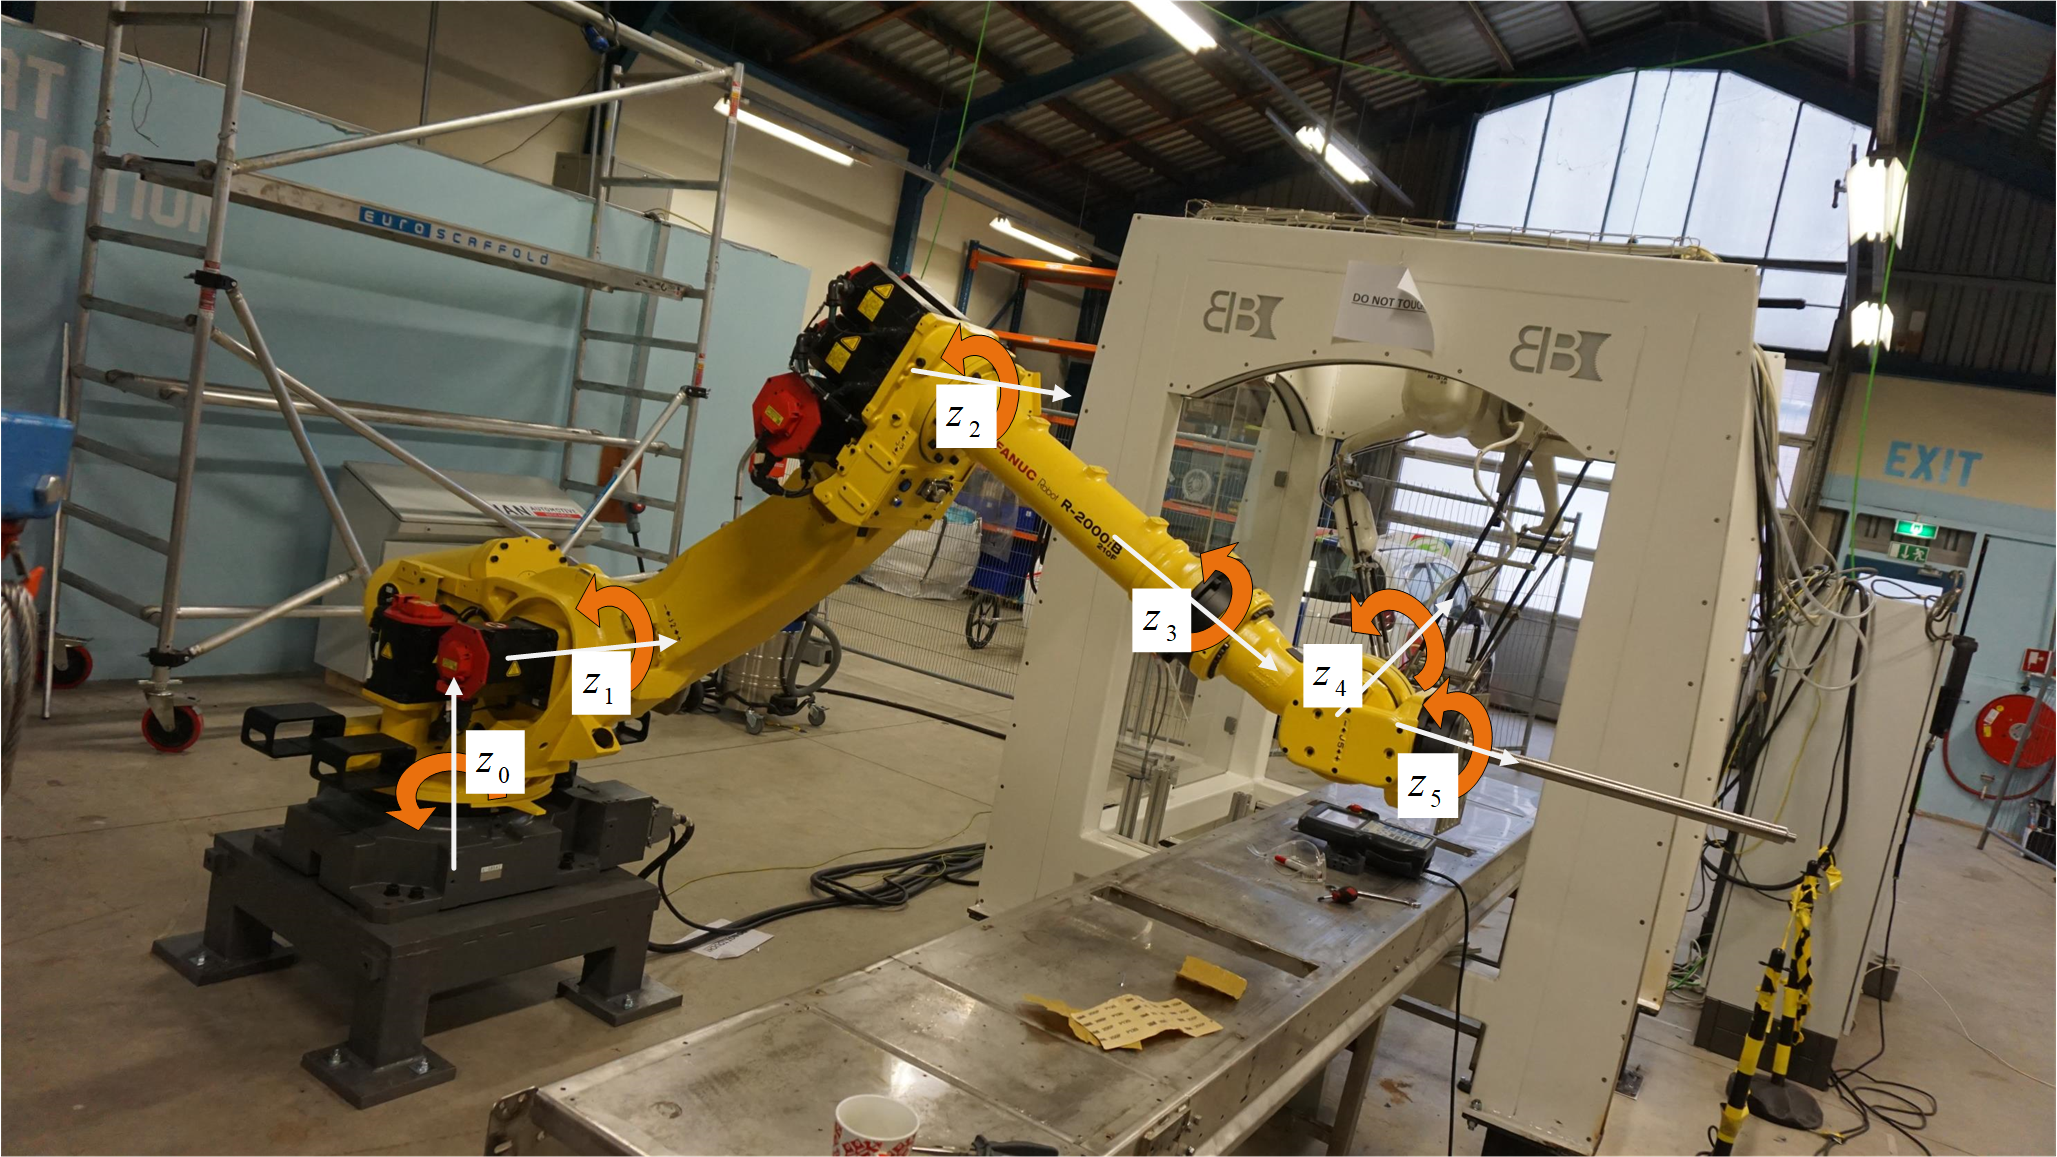
\includegraphics[
	width=1\linewidth,
	center,
	keepaspectratio,
	]{coordinateFrames/z_axes}
	\caption{$z_i$ axes on the Fanuc 210F with the direction of positive rotation (orange)}
	\label{fig:zi_Axes}
\end{figure}


The positive direction of the triples $z_1$, $z_2$, $z_4$ and $z_0$, $z_3$, $z_5$, was chosen to make sure, the x-axis would always have the same direction for parallel joints. 